
%----------------------------------------------------------------------------------------
%	CHAPTER 2
%----------------------------------------------------------------------------------------
\chapterimage{chapter_head_2.pdf} % Chapter heading image

\chapter{\textcolor{red}{Interpretação corporal}}
\label{fig:bodyrelations}

Figura \ref{fig:bodycontroltotal}.

\begin{figure}[!h]
  \centering
    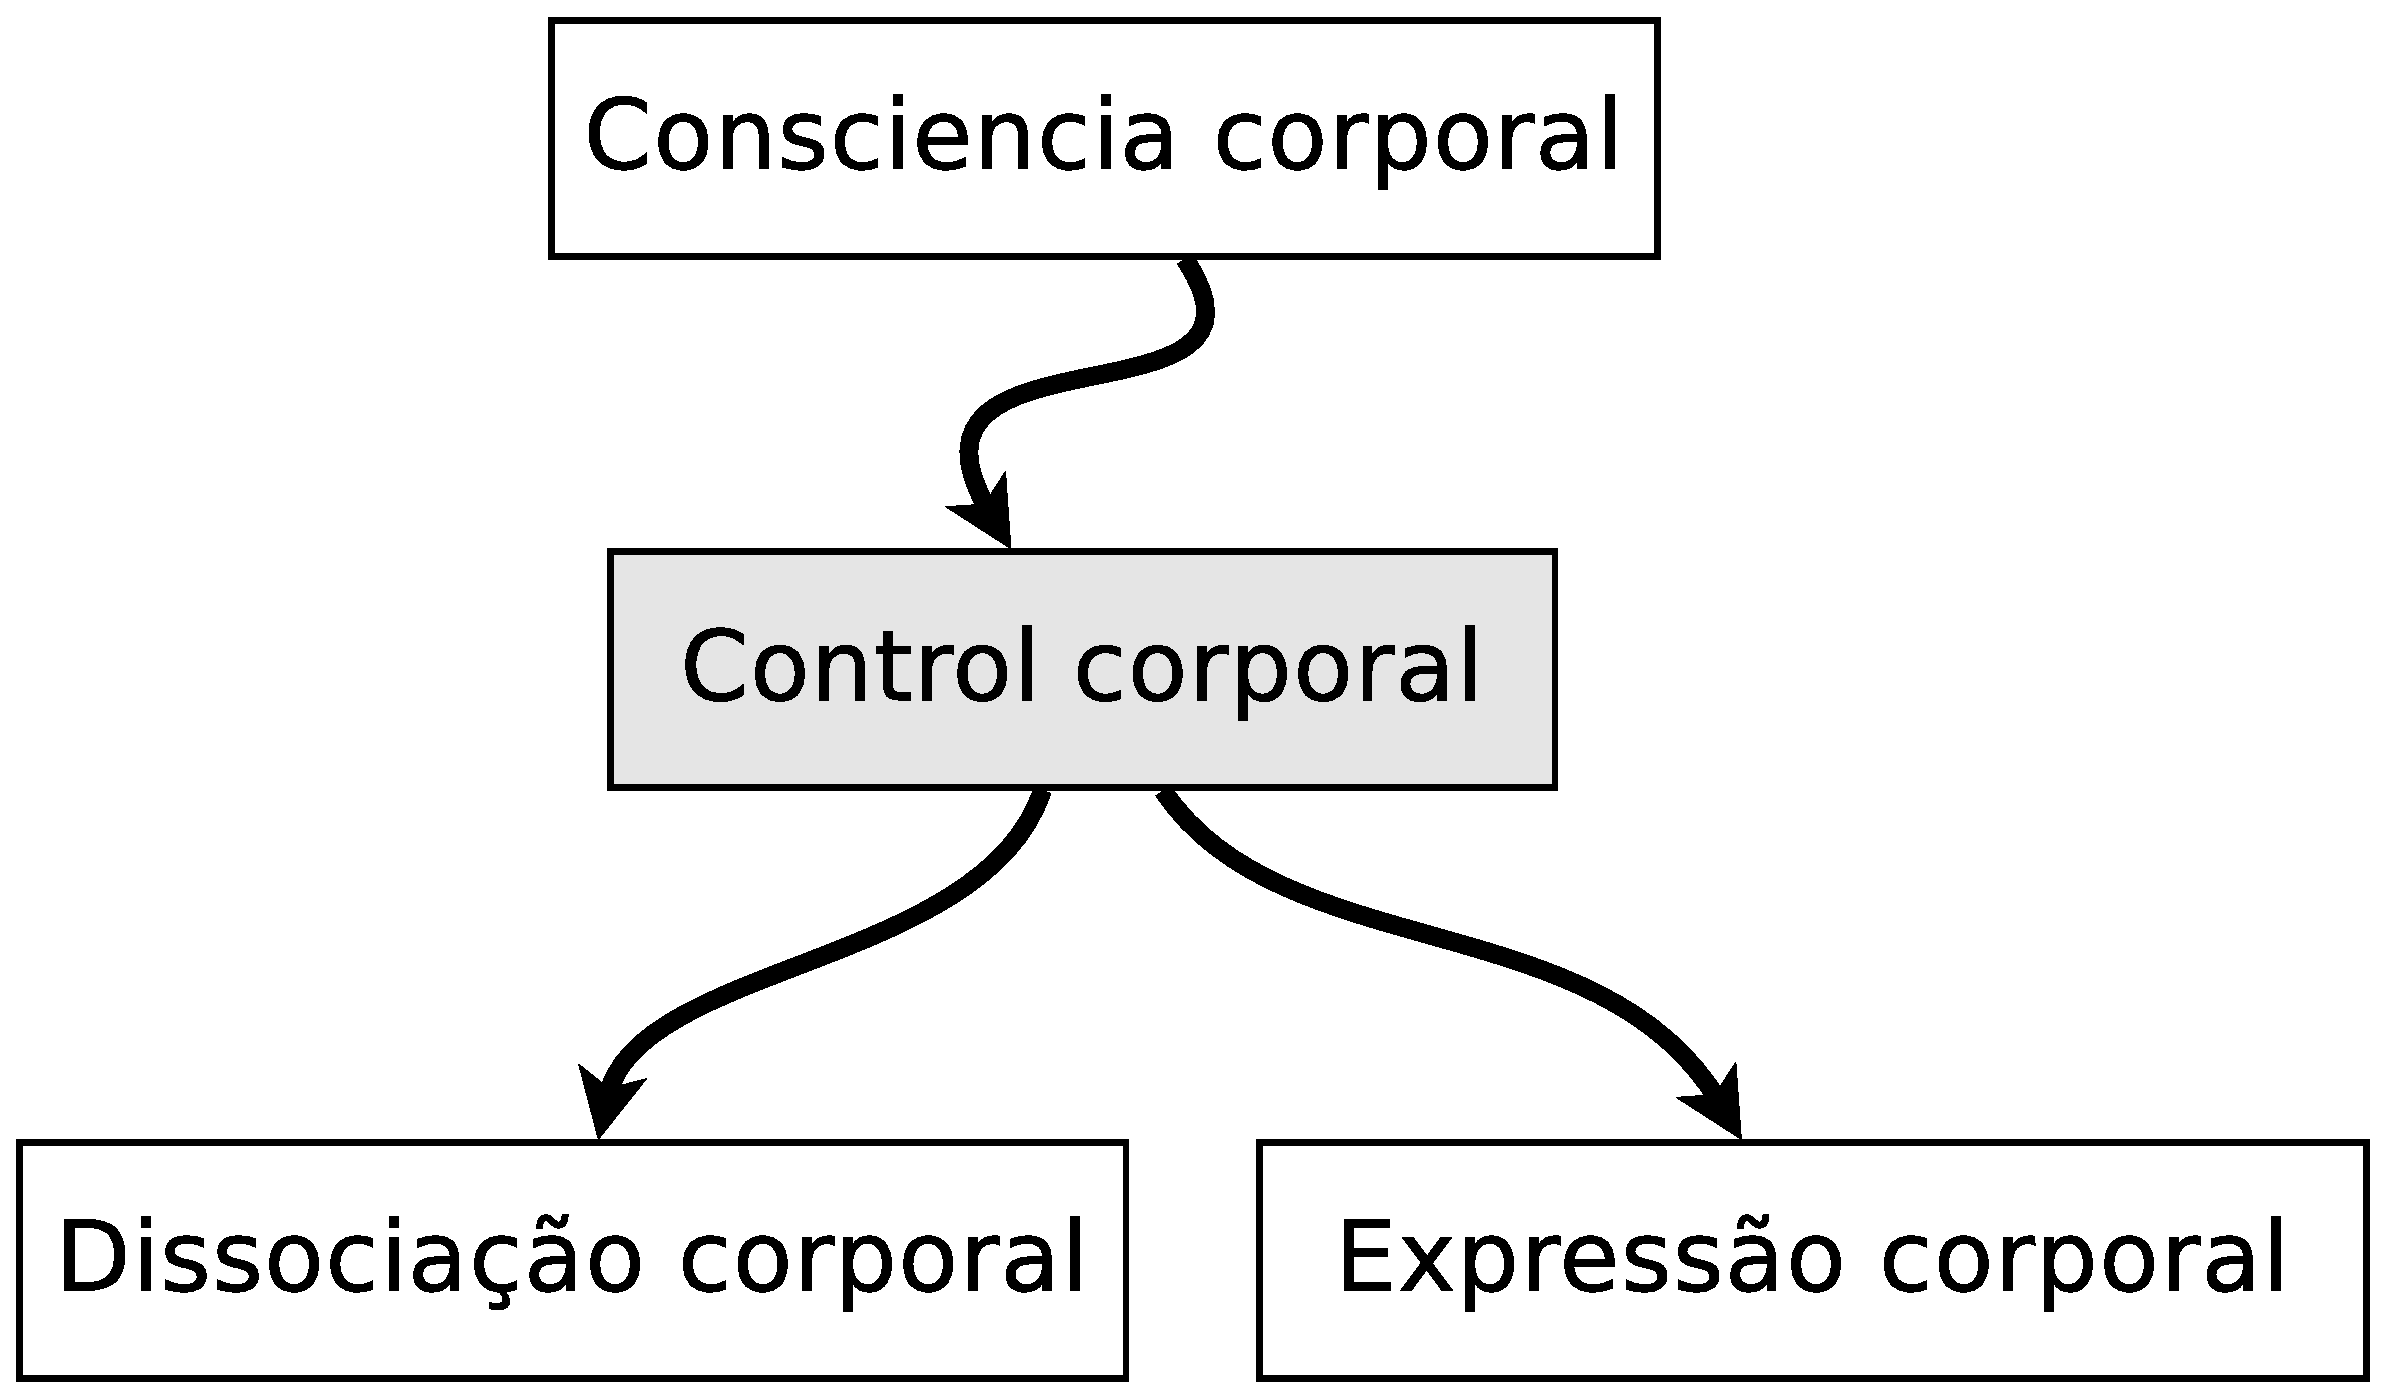
\includegraphics[width=0.5\textwidth]{chapters/cap-body/total.eps}
\caption{Relações do control corporal.}
\label{fig:bodycontroltotal}
\end{figure}


%%%%%%%%%%%%%%%%%%%%%%%%%%%%%%%%%%%%%%%%%%%%%%%%%%%%%%%%%%%%%%%%%%%%%%%%%%%%%%%%
\section{\textcolor{red}{Que é a consciencia corporal?}}
\label{sec:BodyAwareness}
Ou ``Body awareness'' em inglês 
\cite[pp. 11]{balcells2002expresion}
\cite{bueno2016psicomotricidade}
\cite[pp. 232]{gaiarsameio}
\cite[pp. 61]{aranha2002desenvolvimento}
\cite[pp. 75]{vallejo2001cuerpo}

Que o cuerpo está fazendo? \cite[pp. 5]{carline2011lesson} \cite[pp. 27]{paine2014complete}
%%%%%%%%%%%%%%%%%%%%%%%%%%%%%%%%%%%%%%%%%%%%%%%%%%%%%%%%%%%%%%%%%%%%%%%%%%%%%%%%
\section{\textcolor{red}{Que é o \Bodycontrol?}}
\label{sec:BodyControl}
 Ou ``body control'' em inglês 
\cite{bolio2006fantasia}
\cite[pp. 215]{moreno2008expresion}

%%%%%%%%%%%%%%%%%%%%%%%%%%%%%%%%%%%%%%%%%%%%%%%%%%%%%%%%%%%%%%%%%%%%%%%%%%%%%%%%
\section{\textcolor{red}{Que é a expressão corporal?}}
\label{sec:BodyExpression}
\cite{balcells2002expresion}
\cite[pp. 215]{moreno2008expresion}

%%%%%%%%%%%%%%%%%%%%%%%%%%%%%%%%%%%%%%%%%%%%%%%%%%%%%%%%%%%%%%%%%%%%%%%%%%%%%%%%
\section{\textcolor{red}{Que é a \bodyisolation?}}
\label{sec:BodyIsolation}






